\documentclass[]{report}
\newcommand{\home}{C:/Users/ReneNilsson/Documents/GitHub/LaTeX}
\input{\home/Modules/Usepackages}
\input{\home/Modules/ChapterStyle}
\input{\home/Modules/HeaderAndFooter}
\input{\home/Modules/Figure}
\input{\home/Modules/Paragraph}


%FixMe pakken viser små kommentarer, hvor der skal rettes
%--------------------------------------------------
%Brug med følgende: \fxnote{det her skal uddybes!} 
%Se liste over alle fixMe's: \listoffixmes
%Erstat 'draft' med 'final' for at fjerne alle kommentarer
%--------------------------------------------------
\usepackage[footnote,draft,english,silent,nomargin]{fixme}

\begin{document}
\title{Mini Project in TIWSNE}
\author{René Nilsson 10783, Kasper Nielsen 10731, Ivan Grujic 10454, Lasse Pedersen 10769}

\date{\today}
\maketitle
\makeHeaderAndFooter{René Nilsson, Kasper Nielsen, Ivan Grujic, Lasse Pedersen}

\listoffixmes
\tableofcontents

%%!TEX root = TIWSNE_Mini_project_main.tex
Stuff:

\begin{itemize}
\item Overview
  \begin{itemize}
  \item what are we testing
  \item How do we do it
  \end{itemize}
\item Theory
  \begin{itemize}
  \item Compression technique (vs alternatives) 
  \end{itemize}

\item Implementation
\begin{itemize}
\item Sequence from PC $\rightarrow$ mote $\rightarrow$ mote $\rightarrow$ PC
  \begin{itemize}
  \item compressed
  \item uncompressed
  \end{itemize}
\end{itemize}


\item Testing
\item Results
\item Conclusion
\end{itemize}

% Introduction (Ivan)
%!TEX root = TIWSNE_Mini_project_main.tex
\chapter{Introduction}
This report describes a mini project made as part of the masters degree programme in Information Technology at Aarhus University School of Engineering. The project was made in the Wireless Sensor Networks and Electronics course.

Wireless sensor networks consist of a number of battery powered sensor motes, whose operational lifetime is limited by how much energy they consume. In order to extend the lifetime, an effort is put into reducing the energy consumption of the nodes.    

\section{Goal}
The goal of this project is to asses image compression as a method of consuming less energy when transmitting an image from one sensor mote to another. Compressing the image prior to transmission will result in less data being transferred over the air, thereby reducing the energy consumed by the transceiver circuit in both motes. However a reduction in the total energy consumption depends on how much energy is consumed in the compression process.

\section{Description}
This project is concerned with the small sensor network shown in figure \ref{fig:blockDia}. 

\begin{figure}[H]
	\centering
	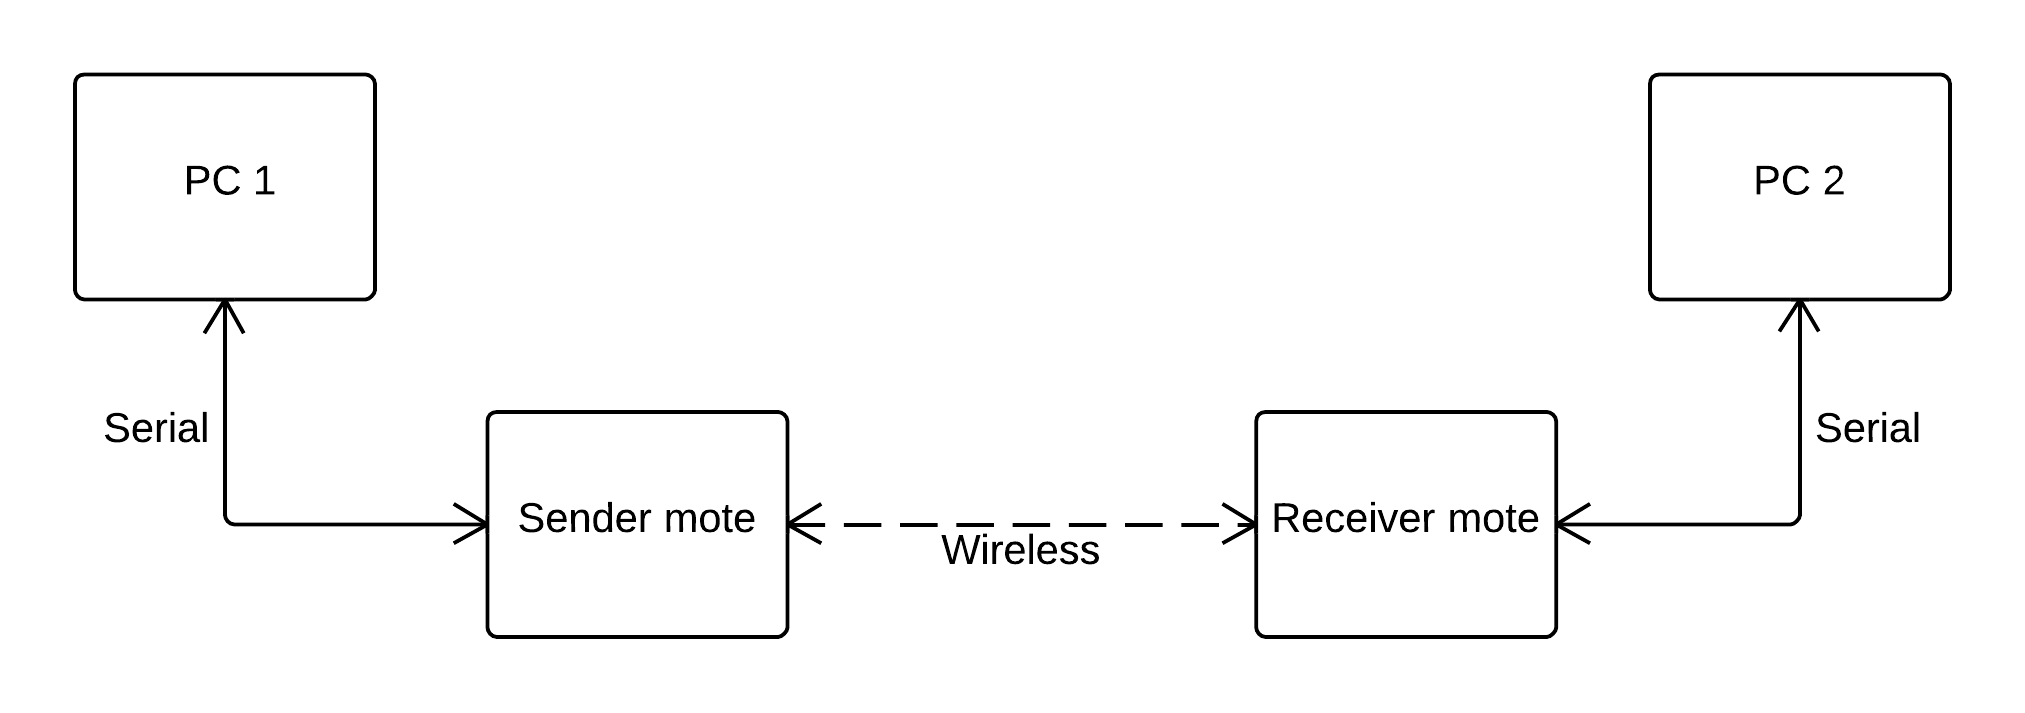
\includegraphics[width=\linewidth, scale = 0.7]{Figures/SimpleBlockDiagram}
	\caption{Block diagram with communication interfaces}
    \label{fig:blockDia}
\end{figure}

The network consists of two motes, a sender mote and a receiver mote, each connected to a PC via a serial connection. An image is loaded onto the sender mote from PC 1, and sent over the wireless channel to the receiver mote, from where it is transferred to PC 2. 
\\Energy consumption measurements of the communication between the motes is to be analysed with and without image compression, to determine its usefulness with regards to saving energy.

The following is to be implemented:
\begin{itemize}
\item A sensor mote application capable of sending and receiving both uncompressed and compressed images over both the wireless and serial channels.
\item A PC application capable of sending and receiving the image to and from the motes.
\end{itemize} 

 

 

% Implementation
%!TEX root = TIWSNE_Mini_project_main.tex
\chapter{Implementation}

%  Wireless (René)
%!TEX root = TIWSNE_Mini_project_main.tex
\section{Wireless transmission}
This project focuses on image compression and energy comparison, but when transmitting data wireless, one must always consider reliability.
Transmission over a wireless channel, is in nature unreliable due to fading, interference, loss of bit synchronization, just to mention some causes.

When dealing with creating a reliable wireless transmission there is two approaches:
\begin{itemize}
\item Automatic Repeat-reQuest (ARQ), which is a reactive approach.
\item Forward Error Control, which is a proactive approach. 
\end{itemize}

The FEC adds redundancy bits to the sent packet and thus decreases the packet error rate. The encoding and decoding requires implementing a block code, such as the Reed-Soloman code. This project does not focus on FEC or block codes, so this approach is discarded. Further it is assumed that the wireless channel is good, and the transmitting distance is very small, so the increased packet error rate might be negligible. The FEC approach alone does not guaranty a error free transmission, it only improves the error rate.

The three most common ARQ methods can be seen in Figure \ref{fig:ARQ}. The Stop and Wait method is the simplest, slowest and most power consuming. The receiver sends a positive acknowledgment for every packet, and the transmitter only transmits one packet at a time. If an acknowledgment is not received within a certain timeout limit, the sender retransmits the last packet.

\begin{figure}
\centering
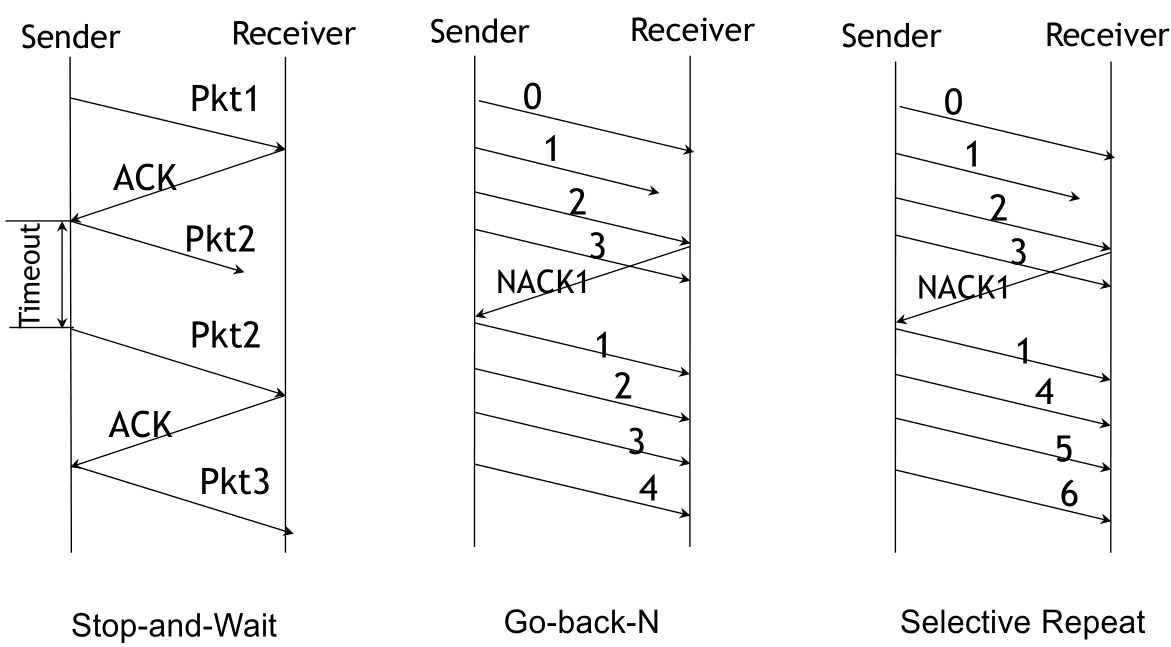
\includegraphics[width=0.7\linewidth]{ARQ}
\caption{Three types of ARQ}
\label{fig:ARQ}
\end{figure}

The last two methods uses negative acknowledgments, which decreases the need for the receiver to transmit packets and thus saves power. The disadvantage is that the sender must keep the last packets send in a buffer, in case a negative acknowledgment is received.

This project focuses on energy comparison and not as much energy savings. Therefore the simplest ARQ method is used : Stop and Wait. An issue when using this method is to find an optimal timeout period. This is a trade off between reducing idle listening and avoiding collisions of acknowledgments and retransmission. The timeout period in this project is set to 100 ms. This has been empirically tested to be more than sufficient to avoid collisions.


%TODO:
Packet size, structs etc.

Sequence numbers.

Error-free
In-sequence
Duplicate-free
Loss-free


%  PC-to-serial (Laze)
%!TEX root = TIWSNE_Mini_project_main.tex
\section{Serial communication}
%sequence diagram for pc-mote.
	%flow control
%mote-pc same as wireless sequence.
%ARQ vs FEC for serial connection.
%check ReliableSerialC
%how to use.

%  Flash handling (Ivan)
\section{Flash Handling}

In order to perform the compression and transmission of the image, the sensor mote must be able to store it in memory. However since Telosb mote uses a Texas Instruments  MSP430 microcontroller with insufficient RAM and internal flash storage\footnote{TelosBProductDescription.pdf\cite{telosbProductDesc} page 1}, the external flash must be used to store the image.

\subsection{Volumes}
When external flash is needed on a sensor mote running TinyOS, the \emph{volume} memory abstraction is available. \cite{tinyOSprog} Since sensor mote application typically do not require high level memory manipulation such a file handling,  it it well suited for deploying sensor mote applications on many different hardware platforms.  

 

   

%!TEX root = TIWSNE_Mini_project_main.tex
\section{Program Flow}
The program deployed on the sender mote and the receiver mote is identical, except for their note id. This is possible, since a state machine is implemented. The main idea is pretty simple. The state machine have eight states, and is controlled with the button on the mote. The LED's on the mote is used to display the current state.


The eight states reflects all the needed functionality in both the sender and receiver:
\begin{itemize}
\item Idle
\item Receiving from PC
\item Sending uncompressed to mote
\item Sending compressed to mote
\item Receiving uncompressed from mote
\item Receiving compressed from mote
\item Sending uncompressed to PC
\item Sending compressed to PC
\end{itemize}

A simplified sequence diagram of the boot sequence and a key press is shown in Figure \ref{fig:BootAndState}. On boot, the used flash areas are erased, and the key is enabled. After boot, the idle state is entered. When the key is pressed the state is changed and everything needed is initialized and the radio is turn on or off, depending on the state. Finally a task is posted to start the transmissions.

\begin{figure}[H]
\centering
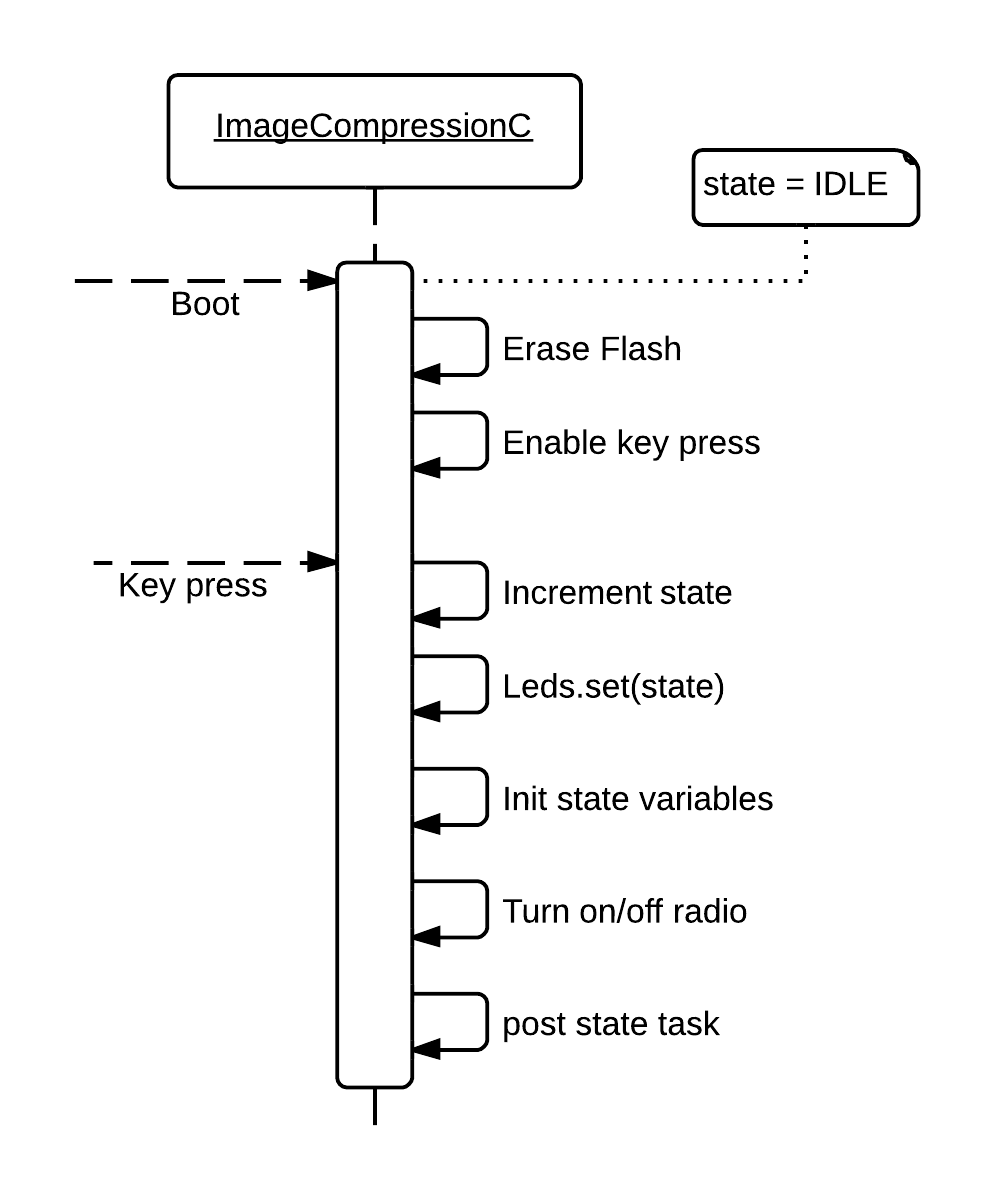
\includegraphics[width=0.5\linewidth]{BootAndStateSeq}
\caption{Simplified boot and state change sequence diagram}
\label{fig:BootAndState}
\end{figure}

In Figure \ref{fig:SendReceiveSeq} a simplified sequence diagram for the \emph{Sending compressed to mote} and \emph{Receiving compressed from mote} states are shown. Each task is initially posted when changing state and executed by the TinyOS. When sending, data is read from the flash, compressed and send. After sending, a timer is started, to be able to retransmit in case no acknowledgment is received. When the ACK is received, the task post itself again. This sequence continues until all packets have been sent, or the state is changed.

The receiving state is quite similar, it waits until it receives a packet, then decompress it and store it in the flash, and sends an ACK back to the sender.


\begin{figure}[H]
\centering
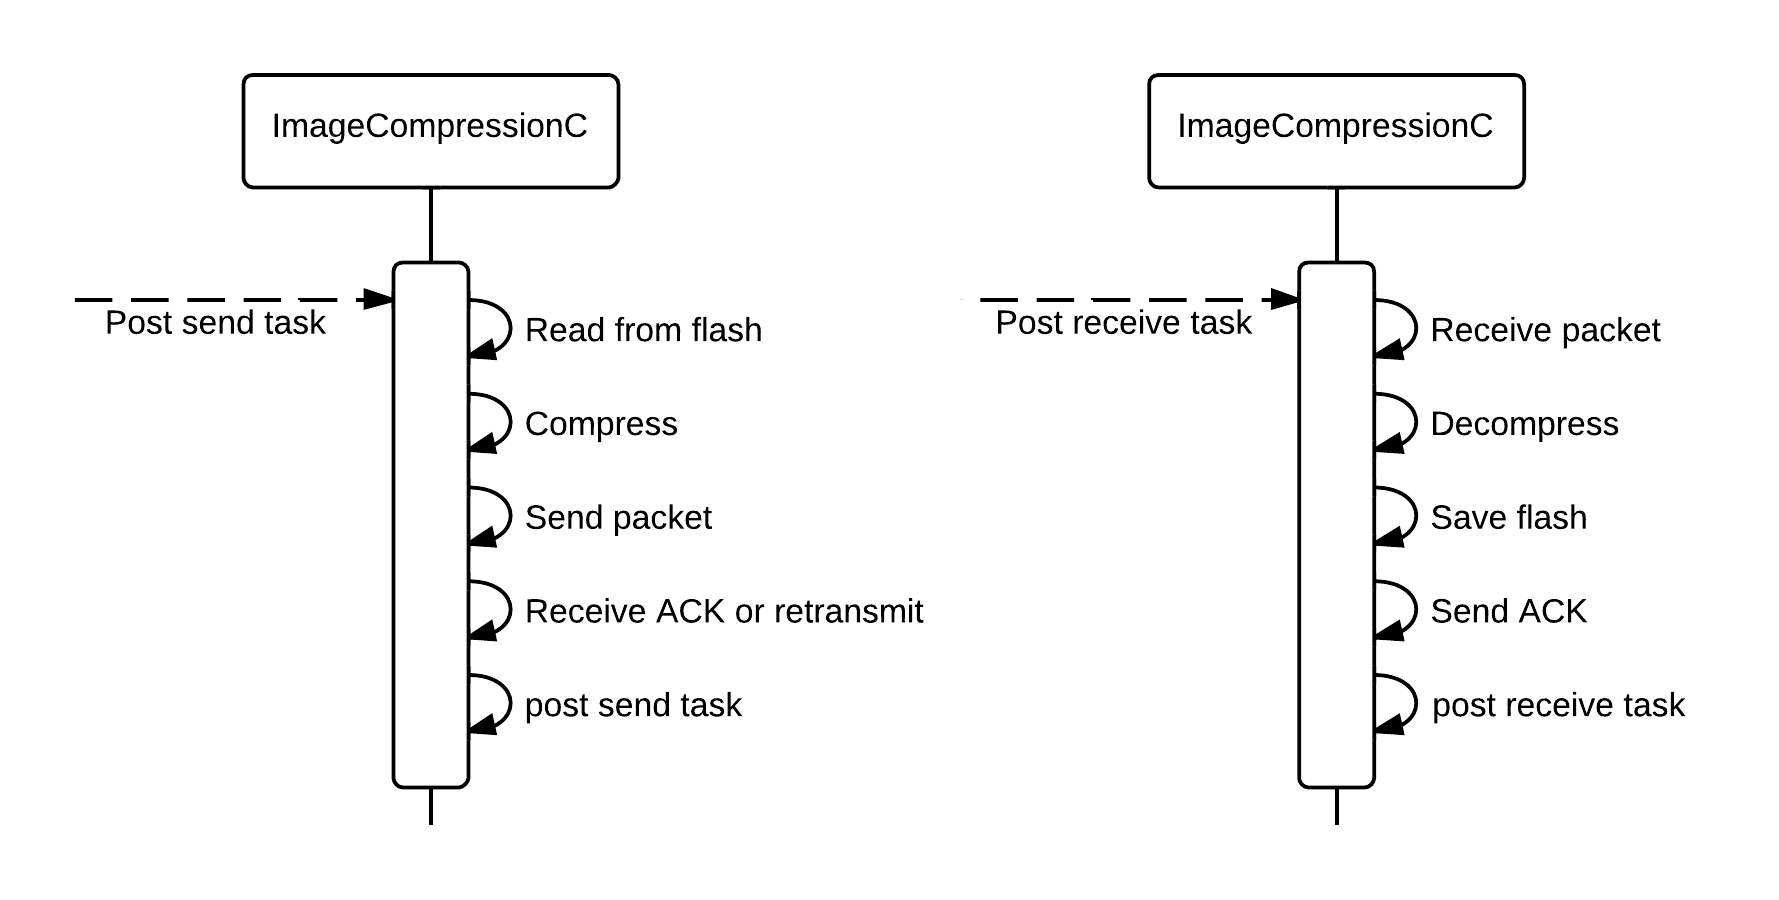
\includegraphics[width=0.9\linewidth]{SendSeq}
\caption{Simplified program flow for wireless transmission.}
\label{fig:SendReceiveSeq}
\end{figure}

The program flow for sending and receiving uncompressed packets, is exactly similar, except that the compression and decompression is removed.

The program flow for communication with the PC is also very similar, except that a serial connection is used instead of the radio.

%  Compression (Kasper)
%!TEX root = TIWSNE_Mini_project_main.tex
\section{Compression}
When compressing an image there are two overall strategies to follow:
\emph{Lossless} or \emph{lossy} compression.

Lossless compression means encoding and repackaging data in order to remove as much redundant information as possible, while maintaining all information needed for a perfect reconstruction. 
One method of doing this is called \emph{Huffman coding}.
This involves building a code tree or "alphabet" with variable symbol length.
Symbols, or our case pixel intensities, that occur more often and hemce contain less information, are encoded with a shorter bit length. 
This increases that average information per symbol, or entropy, leading to a decrease in file size.

The implementation og Huffman coding is rather processor and memory intensive compared to what is available on the TelosB.
Further, an implementation of Huffman coding is beyond the scope of this course.

Instead, a lossy compression scheme has been implemented in this project.
Lossy compression involves discarding information yielding great decreases in file size at the expense of the ability to perfectly reconstruct the image.
An example of lossy image compression is \emph{JPEG-compression}.
This utilizes Discrete Cosine Transforms, knowledge of human psycho-visual perception and ultimately Huffman Coding to greatly compress images while maintaining a low impact on perceived image quality.
Again, this is more processing and memory intensive than what is feasible on a TelosB mote and beyond the scope of the course.

In this project a simple compression scheme has been implemented, where the two least significant  bits (LSB) is truncated, without regard to the amount of information contained within them.
This effectively reduces the amount of data to $ \frac{3}{4} $ of the original. 

Next is the challenge of compressing the truncated data into a smaller bitstream for transmission.
At this point every 6-bit truncated pixel is still stored in a 8-bit \texttt{unit8\_t}.
The way this is handled is by utilizing so-called bitfields.



\fxnote{Insæt exerpt med bitfield struct}
\fxnote{Beskriv imageVector type}

To handle compression and decompression a module has been implemented that provides an \texttt{interface} with \texttt{command}s for each action.
These are then \texttt{call}ed from within the main state machine (See section \ref{sec:program_flow}).



\fxnote{Mere om QuantCompressC, interface og metoder}

%  Program flow (René)


% Results
%!TEX root = TIWSNE_Mini_project_main.tex
\chapter{Results}
%  Image (Laze)
%!TEX root = TIWSNE_Mini_project_main.tex
\section{Image}

The test image was received correctly on the PC. The result can be seen in figure \ref{fig:compressedlena}.

\begin{figure}[H]
\centering
\begin{subfigure}{.5\textwidth}
  \centering
  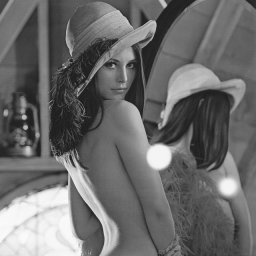
\includegraphics[width=.6\linewidth]{lena}
  \caption{The original, uncompressed test image.}
  \label{fig:lena}
\end{subfigure}%
\begin{subfigure}{.5\textwidth}
  \centering
  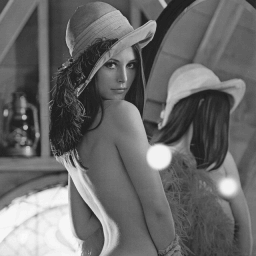
\includegraphics[width=.6\linewidth]{lenacompressed2bit}
  \caption{The test image after being  compressed - 2 least significant bits truncated.}
  \label{fig:compressedlena}
\end{subfigure}
\caption{The test image with and without compression.}
\label{fig:lenacomp}
\end{figure}

As can be seen on figure \ref{fig:lenacomp}, the image resulting from the simple truncation compression is not visibly different from the original image. Thus the reduction in image quality has not been detrimental.

The correctness of the compression was verified by studying the content of the file before and after compression. A comparison of the two files are shown in figure \ref{fig:hexlenacomp}. 

\begin{figure}[H]
\centering
\begin{subfigure}{.5\textwidth}
  \centering
  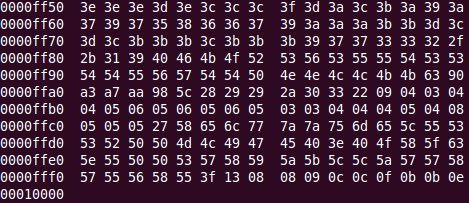
\includegraphics[width=0.95\linewidth]{rawhexdump}
  \caption{Hexdump of the original image.}
  \label{fig:lena}
\end{subfigure}%
\begin{subfigure}{.5\textwidth}
  \centering
  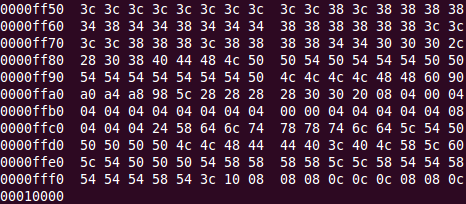
\includegraphics[width=0.95\linewidth]{compressedhexdump}
  \caption{Hexdump of the compressed image.}
  \label{fig:compressedlena}
\end{subfigure}
\caption{Content of the image file with and without compression.}
\label{fig:hexlenacomp}
\end{figure}


%Hexdump
%discussion: harder compression

%  Energy (Kasper)
\section{Energy consumption} 
\label{sec:energy_consumption}
The energy consumptions has been measured for the sending mote.
Measuremens are done by shunting the power supply to measure current draw.
Using an oscilloscope the current draw was integrated over time (See figures \ref{fig:UncompressedSend} and \ref{fig:CompressedSend}).
Then multiplying by the battery voltage yields  energy consumption.

\begin{equation}
E_{send} = 
\dfrac{\int_{}^{}V_{send}\ dt}
{R_{shunt}}
* V_{battery}
\end{equation}

\begin{equation}
R_{shunt} = 10\ \Omega
\qquad
V_{battery} = 2.734\ V
\end{equation}


\subsection{Uncompressed}

\begin{figure}[H]
\centering
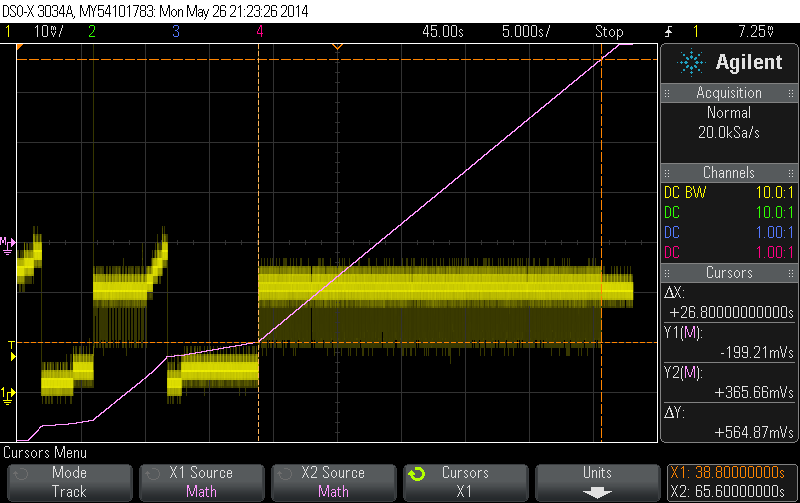
\includegraphics[width=0.8\linewidth]{UncompressedEnergy}
\caption{Voltage over $ 10\ \Omega $ current shunt during sending of an uncompressed image}
\label{fig:UncompressedSend}
\end{figure}

\begin{equation}
E_{send\ Uncompressed} = 
\dfrac{564.87\ mVs}
{10\ \Omega}
* 2.734\ V
=
154.4\ mJ
\end{equation}

\subsection{Compressed}

\begin{figure}[H]
\centering
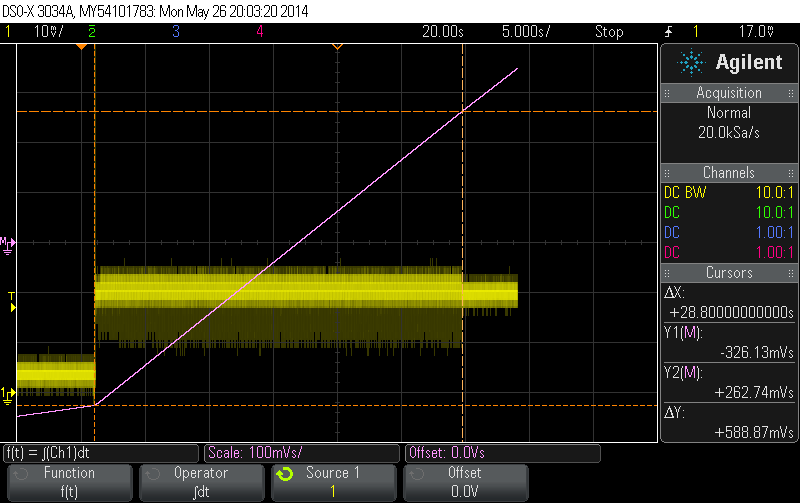
\includegraphics[width=0.8\linewidth]{CompressedEnergy}
\caption{Voltage over $ 10\ \Omega $ current shunt during sending of an compressed image}
\label{fig:CompressedSend}
\end{figure}

\begin{equation}
E_{send\ Uncompressed} = 
\dfrac{588.87\ mVs}
{10\ \Omega}
* 2.734\ V
=
160.99\ mJ
\end{equation}





% Discussion (All)
%!TEX root = TIWSNE_Mini_project_main.tex
\chapter{Discussion}

\section{Energy considerations}

The thesis for this project is that energy could be saved, by compressing data before transmitting it. As it is represented in the results, this is not the case for this project. The main reason for this is a faulty application design. 
The theory states that energy can be saved, because compressing and decompressing data consumes much less power than is saved by transmitting fever packets.

However, in our design, the compression and decompression takes place while the radio is turned on. In this way no power is saved. On the contrary it uses more power.

Unfortunately we did not have the time to correct the design and prove the theory, but a short reasoning supports the theory:


\fxnote{Check all values!}
In the results, it was shown that transmitting all the uncompressed data took 26 seconds. In the case with compression it took 28.6 seconds, even though 20\% fever packets where sent. 

If the compression happened prior to the transmission, sending the compressed data would roughly take $26*0,80 = 20.8$ seconds. 

Compressing the data prior to the transmission might increase the time used, due to increased flash handling, but we will assume it takes 10 seconds.
When the radio is turned of, the current draw from the mote is approx. 3 mA. When the radio is on it is 20 mA. 
% Perhaps we should use watt instead?

Using these metrics we can calculate the used consumption in both cases:\\
Uncompressed:
\begin{equation}
26 s * 20 mA = 520 mAs
\end{equation}
Compression prior to transmission:
\begin{equation}
10 s * 3 mA + 20.8 s * 20 mA = 30 mAs + 416 mAs  = 446 mA
\end{equation}

From these calculations there is a clear power saving, by performing the compression. Even though these are all rough estimates, changing the parameters slightly to the worse, will not change the result.

Note that this is only based on the sending mote, but the calculations for the receiving mote will be very similar, since transmitting and receiving uses almost the same power. 

\section{Compression rate}

The compressed image did not visibly loose quality, thus harder compression (truncating more bits) would be possible while still maintaining an acceptable image quality - depending on the application requirements.
Truncating 4 bits instead of two would effectively halve the data to be sent.
Using 4 bits would also significantly reduce the complexity of the compression algorithm, as $4 \texttt{ bits} * 2= 1 \texttt{ octet}$ and the radio interface is octet based.
The approach used in the project packs $5 * 6\texttt{ bits} = 30\texttt{ bits}$ in $32 \texttt{ bit}$ chunks thus wasting $\frac{2\texttt{ bits}}{32\texttt{ bits}}*100\% = 6.25\%$ of transmitted data.

\section{Design Improvements}

Given the above calculations and aforementioned results, a number of design improvements are suggested: 

\begin{enumerate}
\item When sending, the application should be modified to put the transceiver circuit in sleep mode when not transmitting a package. 
\item When receiving, the application should be modified to send the acknowledgement as soon as the packet has been received.
\item Using a compression, which doesn't result in wasted bits being transmitted. 
\end{enumerate} 

If timing control was added to the wireless protocol, it would be possible to put the receiving radio circuit in sleep mode whilst decompressing and storing the packet. The mote should then use the timing information to know when to turn the radio back on and listen for the next packet.

The improvements are concerned with reducing the amount of time spent with the transceiver circuit turned on, as this part of the mote consumes a lot of energy.  

%  Stikord fra alle


% Conclusion (All)
%!TEX root = TIWSNE_Mini_project_main.tex
\chapter{Conclusion}

Based on the results and discussion chapters it can be concluded that this project does not conclusively confirm that image compression will reduce power consumption in a sensor network. However considering the calculations and design improvements presented in the discussion, compression can still be argued as a good approach to reducing energy consumption. Even though the results of this project do not verify this claim, this is due to the 

\chapter{Appendix}

\begin{enumerate}
\item Source code for the sensor more application can be found in ImageCompressionSource.zip  \label{App:SourceCode}
\item Source code for the PC serial application can be found in PCFileTransferer.zip 
\end{enumerate}

\begin{thebibliography}{9}
\addcontentsline{toc}{chapter}{Bibliography}

\bibitem{telosbProductDesc}	
Moteiv Corporation, \emph{TelosB ProductDescription.pdf}, 2004

\bibitem{tinyOSprog}
Levis, Philip, and David Gay. \emph{TinyOS programming} Cambridge University Press, 2009.

\end{thebibliography}

\end{document}